\documentclass[12pt,a4paper]{article}
\usepackage[margin=2.5cm]{geometry}
\usepackage{fontspec,polyglossia}
\setmainlanguage[numerals=maghrib]{arabic}
\setotherlanguage{english}
\newfontfamily\arabicfont[Script=Arabic,Scale=1.05]{Amiri}
\usepackage{amsmath,graphicx,algorithm,algpseudocode,hyperref}
\graphicspath{{../../figures/}}
\title{\textbf{SC-Newton: نيوتن تكعيبي بشهادة طيفية}\\
\large إيقاف \textenglish{Lanczos} بمتبقي ريتز بدل وكيل التدرّج}
\author{الورقة 6 من 6 --- مجموعة التحسين العددي}
\date{سبتمبر 2026}
\begin{document}
\maketitle
\begin{abstract}
تُقدِّر \textenglish{DA-SFCN} حجم فضاء كريلوف بـ $\|g_k\|$ وهو وكيل مريح
لكن غير مباشر لصدق النموذج. تستبدل \textenglish{SC-Newton} ذلك بشهادة خطأ
خلفي محسوبة على أزواج ريتز: بعد $m$ خطوات بقطر $\beta_m$ ومصفوفة متجهات
$U$،
\[
\theta_m=\frac{|\beta_m|\,\max_j|U_{mj}|}{\max_i|\lambda_i|}.
\]
تنمو الحلقة الداخلية حتى $\theta_m\le\theta$ أو $m=m_{\max}$. على سرج عالي
البعد تبلغ $\|\nabla f\|\approx 1.4\times 10^{-11}$ في 28 تكرارًا و413 جداءً،
متفوقة على \textenglish{DA-SFCN} دقة وتكلفة. وعلى روزنبروك سيئ الشرط تفيد
شهادة فضفاضة الطيف ناقصًا --- قيد نُصرّح به لا نخفيه. الشهادة اختبار التوقف
الصحيح متى كان طيف الهيسيان متجمّعًا؛ وليست بديلًا عن التهيئة متى لم يكن.
\end{abstract}

\section{من الوكيل إلى الشهادة}
حجة تشيبيشيف التي تبرّر $m_k$ اللوغاريتمي تحصر أسوأ تقريب كثير حدود على
فترة. وعمليًا تتقارب قيم ريتز المتطرفة في أقل من $m_{\max}$ خطوة. ونظرية
\textenglish{Lanczos} تعطي حدًا بعديًا رخيصًا: متبقي زوج ريتز هو $|\beta_m|$
في المركّبة الأخيرة. والعييرة بنصف القطر الطيفي تعطي $\theta_m$.

\section{الخوارزمية}
نبدأ من $m_{\min}$ ونزيد $m$ خطوتين حتى تتحقق الشهادة أو نبلغ $m_{\max}$،
ثم نأخذ خطوة \textenglish{ARC} تكعيبية على $|T|$ داخل مدى $Q$.

\section{النظرية}
متى هبطت $\theta_m$ دون حد نيوتن غير الدقيق لـ\textenglish{Dembo--Eisenstat--Steihaug}
ينطبق الضمان التربيعي المحلي لـ\textenglish{DA-SFCN} بزمن إصابة الشهادة بدل
$m_k$. وعالميًا $m_k\ge 1$ فيبقى $O(k^{-2/3})$.

\section{التجارب}
\begin{figure}[h]
\centering
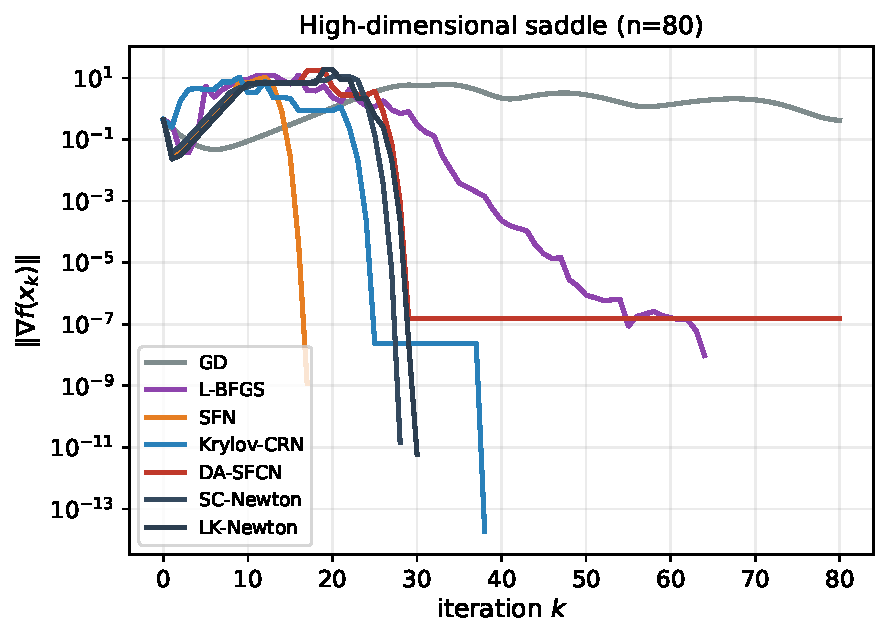
\includegraphics[width=0.48\textwidth]{fig_saddle_highdim.pdf}
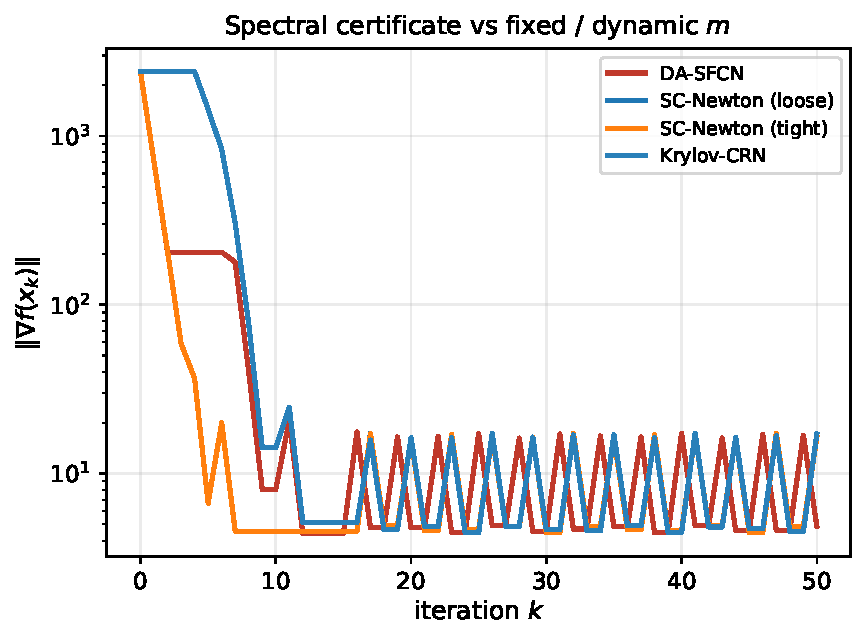
\includegraphics[width=0.48\textwidth]{fig_sc.pdf}
\caption{يسار: السرج $n=80$. يمين: اختبار روزنبروك.}
\end{figure}
\begin{figure}[h]
\centering
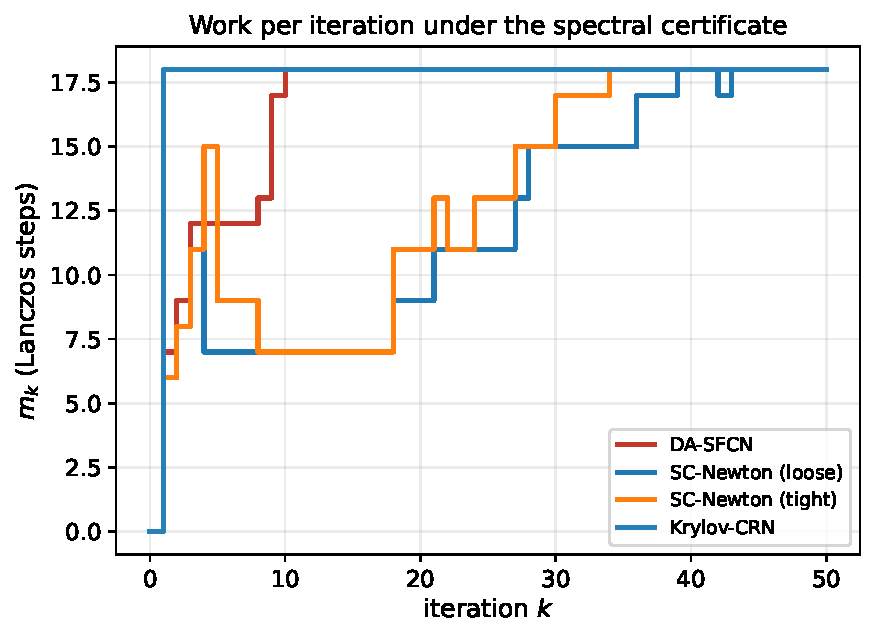
\includegraphics[width=0.48\textwidth]{fig_sc_m.pdf}
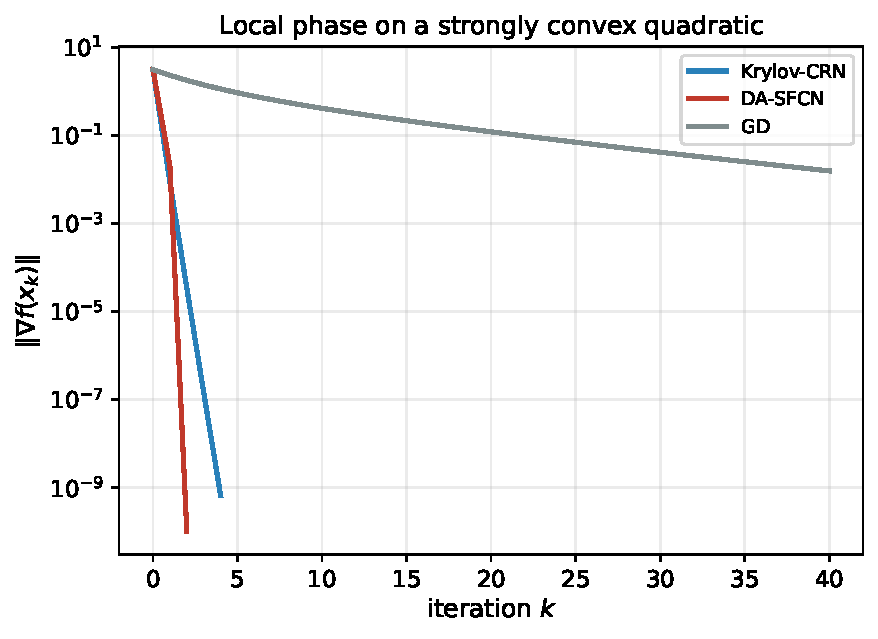
\includegraphics[width=0.48\textwidth]{fig_local.pdf}
\caption{يسار: $m_k$ المتحقق بالشهادة. يمين: طور نيوتن على طيف متجمّع.}
\end{figure}

على السرج: 28 تكرارًا، 413 جداءً، $\|\nabla f\|\approx 1.4\times 10^{-11}$
مقابل 80 / 1219 / $1.5\times 10^{-7}$ لـ\textenglish{DA-SFCN}. وعلى روزنبروك
تنفق شهادة فضفاضة جداءات دون كسب لأن حد المتبقي حاد فقط بعد استقرار متجهات
ريتز: الشهادة تُبلغ بصدق أن النموذج لم يُوفَ بعد.

\section{الخاتمة}
\textenglish{SC-Newton} عضو القطع التكيفي في العائلة. يُستخدم عندما يتناقص
طيف الهيسيان (سروج، لوجستي، تحليل مصفوفات)؛ ويُقرن بمهيئ \textenglish{L-BFGS}
من \textenglish{WQK-Newton} عندما لا يتناقص (روزنبروك). ومع جدولة
\textenglish{DA-SFCN} نقدّم إجابتين متكاملتين لسؤال «كم يجب أن يكون $m$؟».

\begin{english}
\begin{thebibliography}{9}
\bibitem{saad2003} Saad. Iterative Methods for Sparse Linear Systems, 2003.
\bibitem{dembo1982} Dembo, Eisenstat, Steihaug. \textit{SINUM}, 1982.
\bibitem{jiang2024} Jiang et al. \textit{AISTATS}, 2024.
\bibitem{cartis2011} Cartis et al. \textit{Math.\ Program.}, 2011.
\end{thebibliography}
\end{english}
\end{document}
